\cotefile{85}
\scanpage{72}
\[
 \boxed{\deleted{(5,5,3)}}\qquad
 \theta_0=\theta_1=\frac{2\pi}{5}\qquad \theta=\frac{2\pi}{3}
\]

\[
\begin{aligned}
\cos\frac{\theta_0-\theta_1}{2}&=\cos(\theta_0-\theta_1)=1\\
\deleted{\unsure{\cos|\sin|2}}\unsure{\sin|\cos}\theta&=-1\qquad
 \sin\frac{\theta_0}{2}=\sin\frac{\theta_1}{2}\overset{?}{=}\sin\frac{\pi}{5}
 =\deleted{\unsure{\sqrt{\tfrac12(\alpha+1)}}}\\
\sin^2\frac{\theta_0}{2}&=\tfrac12(\deleted{\unsure{\cos\theta_0}}1-\cos\theta_0)
 =\tfrac12(1-\tfrac{\alpha}{2})=\tfrac14(2-\alpha)\\
\sin^4\frac{\theta_0}{2}&=\tfrac1{16}\underbrace{(\alpha^2+4-4\alpha)}_{5-5\alpha}=\tfrac5{16}(1-\alpha)
\end{aligned}
\]

\[
 \frac1{|1+\zeta|}\Re(1+\zeta)=\sin\frac{\pi}{5}
\]

\figure{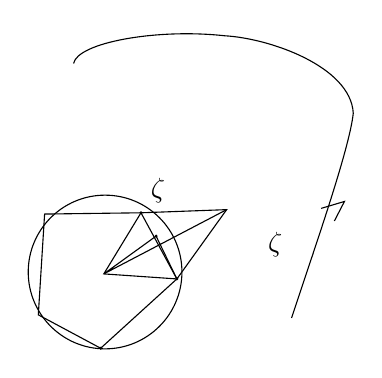
\begin{tikzpicture}[scale=.8,thin]
\coordinate (O) at (0,0);
\draw (.02,.03) circle (1.22);
\draw (-.94,.95)--(.59,.97)--(1.16,-.08)--(-.05,-1.18)--(-1.04,-.65)--cycle;
\draw (O)--(.59,.97) node[above right] {$\zeta$}--(1.95,1.02)--(1.16,-.08)--cycle;
\draw (O)--(1.95,1.02) (O)--(.83,.60)--(1.16,-.08);
\foreach \x/\y in {.59/.97,.83/.60,1.16/-.08,-.05/-1.18}{\fill (\x,\y) circle (.026);}
\node at (2.72,.47) {$\zeta$};
\draw (2.98,-.70) .. controls (3.33,.36) and (3.90,1.98) .. (3.96,2.55)
 .. controls (3.92,3.29) and (2.64,3.74) .. (1.92,3.78)
 .. controls (.83,3.90) and (-.42,3.67) .. (-.48,3.34);
\draw (3.45,1.04)--(3.82,1.15)--(3.66,.84);
\end{tikzpicture}}

\[
\begin{aligned}
{\unsure{\xi|\zeta}}^2-\frac1{\sin^2\frac{\pi}{5}}\xi
 +\frac18\frac{1-(-1)}{\sin^4\frac{\pi}{5}}&=0\\
\text{\unsure{i.e}} \qquad
 \xi^2-\frac1{\tfrac14(\unsure{2-\alpha|2+\alpha})}\xi
 +\frac14\frac1{5/16(1-\alpha)}&=0
\end{aligned}
\]

\[
 \zeta=\alpha/2+i\underbrace{\sqrt{1-\frac{\alpha^2}{4}}}_{1/2\sqrt{4-\alpha^2}}
 =\alpha/2+i/2\sqrt{\alpha+3}
\]

\[
 \deleted{\alpha^2+\alpha-1=0}\qquad \uline{NB}\qquad 4-\alpha^2=3+\alpha
\]

\[
 \xi^2-\frac{4(2-\alpha')}{(2-\alpha)(2-\alpha')}\xi
 +\frac45\frac{(1-\alpha')}{(1-\alpha)(1-\alpha')}
\]

\[
\begin{aligned}
 |\zeta+1|^2&=(1+\alpha/2)^2+\left(\frac{\sqrt{\alpha+3}}2\right)^2\\
 &=1+\alpha+\underbrace{\frac{\alpha^2}4+\frac{\alpha+3}4}_{\unsure{1/2|1}}\\
 &=\frac32+\alpha+
\end{aligned}
\]

\[
\begin{aligned}
N(2-\alpha)&=4-1+2=5\\
N(1-\alpha)&=1-1+1=1\\
-\alpha'&=+1+\alpha\\
2-\alpha'&=3+\alpha\\
1-\alpha'&=2+\alpha
\end{aligned}
\]

\[
 \sin\frac{\pi}{5}=\frac{1+\alpha/2}{\sqrt{3/2+\alpha}}
 =\deleted{\unsure{\tfrac12|\tfrac14}}\frac{(\alpha+2)}{3+2\alpha}\sqrt{3/2+\alpha}
 =\alpha\sqrt{3/2+\alpha}=\deleted{\unsure{\sqrt{(3/2)\alpha^2+\alpha^2}}}
\]

\[
 \underbrace{N(3+2\alpha)}_{\shortparallel\ (3+2\alpha)(3+2\alpha')}=9\unsure{-|+}\deleted{\unsure{4}}4-6=-1
\]

\[
\begin{aligned}
 \sin^2\left(\frac{\pi}{5}\right)&=\alpha^2(3/2+\alpha)=(1-\alpha)(3/2+\alpha)\\
 &=3/2-1/2\,\alpha\underbrace{-\alpha^2}_{\alpha-1}=\tfrac12(\alpha+1)
\end{aligned}
\]

\[
\begin{aligned}
 \frac{\alpha+2}{3+2\alpha}&=-(\alpha+2)(3+2\alpha')=-(\alpha+2)(1-2\alpha)\\
 &=-[\underbrace{-2\alpha^2}_{2\alpha-2}-3\alpha+2]=\alpha
\end{aligned}
\]

\[
 \deleted{\unsure{\xi^2-}}
\]

\[
\begin{aligned}
 \xi^2-\left[\tfrac45(3+\alpha)\right]\xi+\left(\tfrac45(2+\alpha)\right)&=0\\
 \xi=\tfrac{\deleted{\unsure{4}}2}{5}(3+\alpha)
 \mathbin{\pm}\tfrac25\sqrt{\deleted{\unsure{\tfrac4{25}}}(3+\alpha)^2-
 \deleted{\unsure{\tfrac15}}5(2+\alpha)}
 &=\tfrac25(3+\alpha)\mathbin{\pm}\sqrt{-5\alpha}
\end{aligned}
\]

\[
 \deleted{\unsure{28}}\qquad
 \deleted{9}+6\alpha+\underbrace{\alpha^2}_{\deleted{1}-\alpha}-\deleted{10}
 -\unsure{15|5}\alpha=\deleted{\unsure{-5\alpha|5\alpha}}
\]
% archive sheet number: 71
